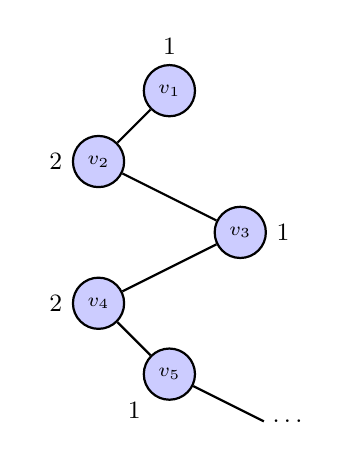
\begin{tikzpicture}[
  baseline=0pt,
  scale=1,
  vnode/.style={circle, draw=black, fill=blue!20, thick, inner sep=0pt, minimum size=6.5mm},
  edge/.style={thick, draw=black},
  clabel/.style={font=\small, color=black}
]
  % Caja delimitadora simétrica (-1.8 a 1.8) para centrar el eje x = 0
  \useasboundingbox (-1.8,-2.8) rectangle (1.8,2.4);

  \begin{scope}[yshift=-0.2cm]
    % Primeros 5 vértices
    \node[vnode, label={[clabel]above:$1$}]        (v1) at (0.0, 1.8) {$\scriptstyle v_1$};
    \node[vnode, label={[clabel]left:$2$}]         (v2) at (-0.9, 0.9) {$\scriptstyle v_2$};
    \node[vnode, label={[clabel]right:$1$}]        (v3) at (0.9, 0.0) {$\scriptstyle v_3$};
    \node[vnode, label={[clabel]left:$2$}]         (v4) at (-0.9, -0.9) {$\scriptstyle v_4$};
    \node[vnode, label={[clabel]below left:$1$}] (v5) at (0.0, -1.8) {$\scriptstyle v_5$};

    % Aristas
    \draw[edge] (v1) -- (v2) -- (v3) -- (v4) -- (v5);
    \draw[edge] (v5) -- (1.2, -2.4);
    \node[font=\small] at (1.5, -2.4) {$\dots$};
  \end{scope}
\end{tikzpicture}
